\author{Emanuele Carraro}

\title{Project report for Bioinformatics course}
\maketitle

\newpage
\tableofcontents

\newpage
\section{Project report}

In the directory you will find the genomic reference sequence of a bacterium
called Lactobacillus casei. The genome is \texttt{3,079,196} bp long.

The aim of the project is the ``resequencing'' of a similar
bacterium that we call lact.sp, using mate pairs reads.

In particular we want to see if lact.sp has genomic structural variations.

We suspect that the lact.sp genome may have small and large deletions,
insertions and inversions, and we want to find where they are.

The mate pairs fastq reads are supplied in two files.
\subsection{Part 1}

\begin{enumerate}
\item Download the reference genome and the zip file with the fastq reads
\item Install BWA on your computer
\item Use BWA to align the illumina reads on the reference genome
\item Install IGV on your computer
\item Process the sam file obtained by the BWA analysis to make a bam file
\item Sort and index the bam file (see unix.pdf)
\item Visualize the coverage and mate pairs on the IGV
\item Manually find and comment any ``anomalous'' pair of mates
\end{enumerate}

\subsection{Part 1 - Answers}
\begin{enumerate}
  \item This part was done in classroom
  \item This part was done in classroom
  \item Enter the following command in the directory with the reads and the
reference genome: \texttt{bwa index Lactobacillus\_casei\_genome.fasta} and
\texttt{bwa mem Lactobacillus\_casei\_genome.fasta lact\_sp.read1.fastq 
lact\_sp.read2.fastq > lact\_sp.sam}
  \item This part was done in classroom
  \item Enter the following command:
\texttt{samtools view -bS lact\_sp.sam > lact.bam}
  \item Enter the following command:
\texttt{samtools sort lact.bam lact\_sorted} and
\texttt{samtools index lact\_sorted.bam}
  \item In figure \ref{fig:coverage_matepairs} there is a screen of IVG
interface with the coverage (\texttt{lact\_sorted.bam.Coverage}) and mate pairs
(\texttt{lact\_sorted.bam})

\begin{figure}[h]
  \centering
  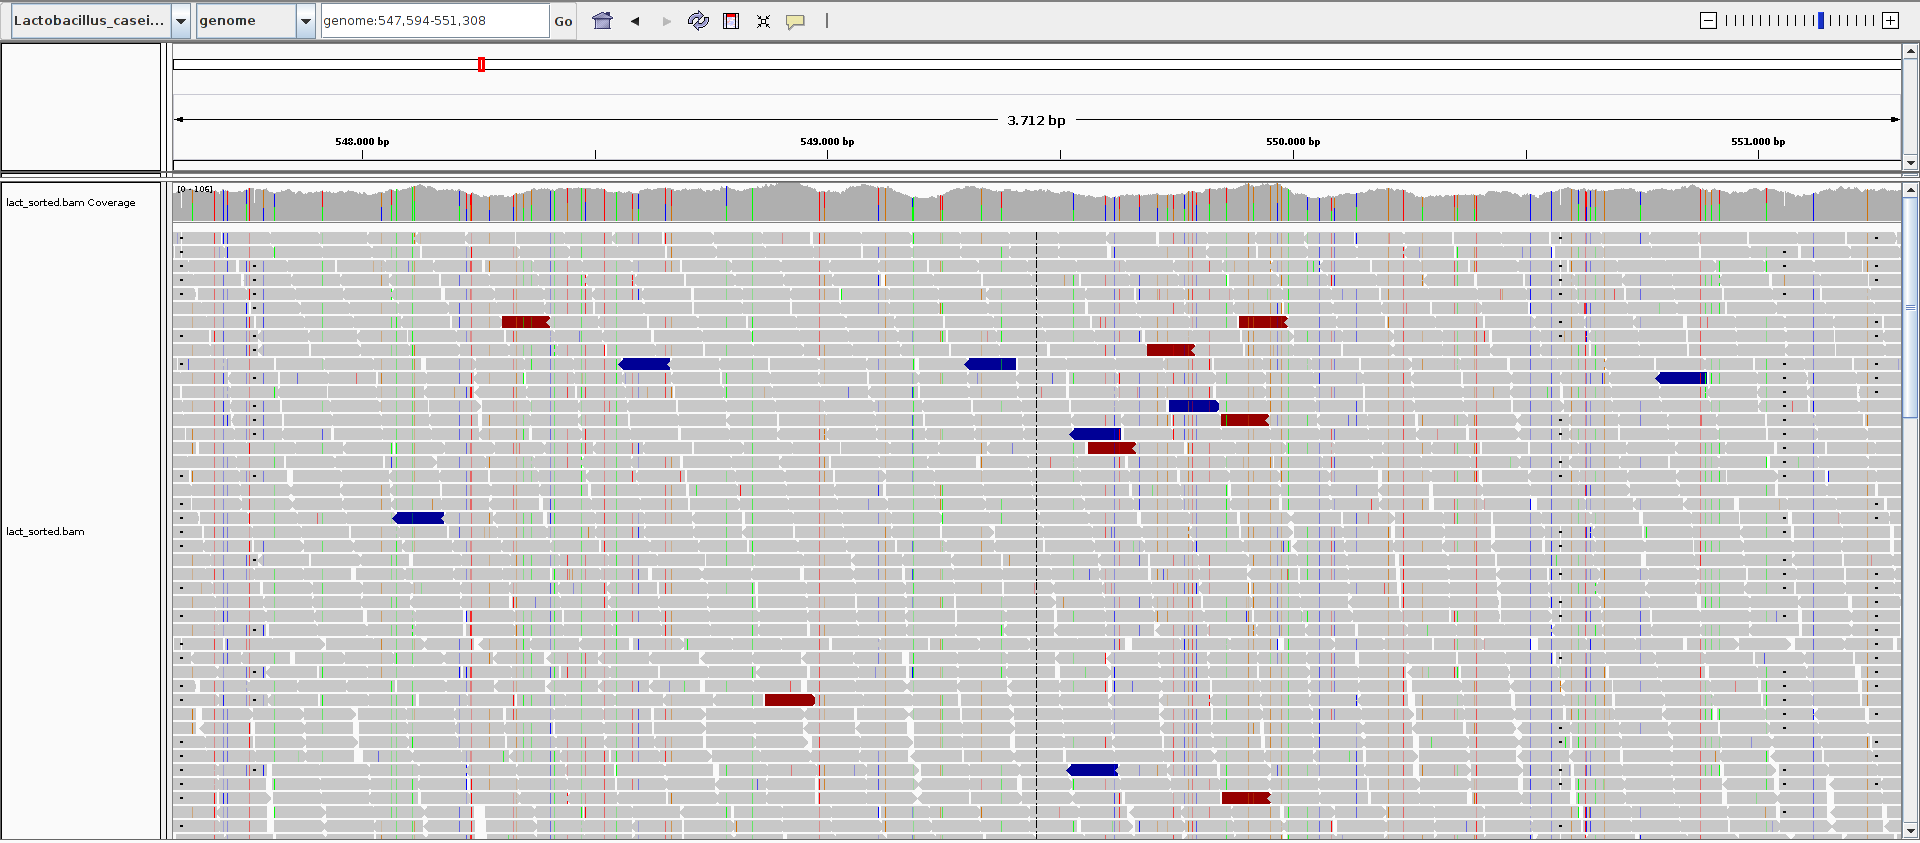
\includegraphics[scale=0.2]{img/coverage_matepairs}
  \caption{Coverage and mate pairs on the IGV}
  \label{fig:coverage_matepairs}
\end{figure}

  \item In the following examples I used some of the wiggle files produced in
part 2 of the practicals because they help in finding structural variations.

\textbf{Examples}: \\

It can be observed that in figure \ref{fig:pairs} there is
a long deletion.

\begin{figure}[h]
  \centering
  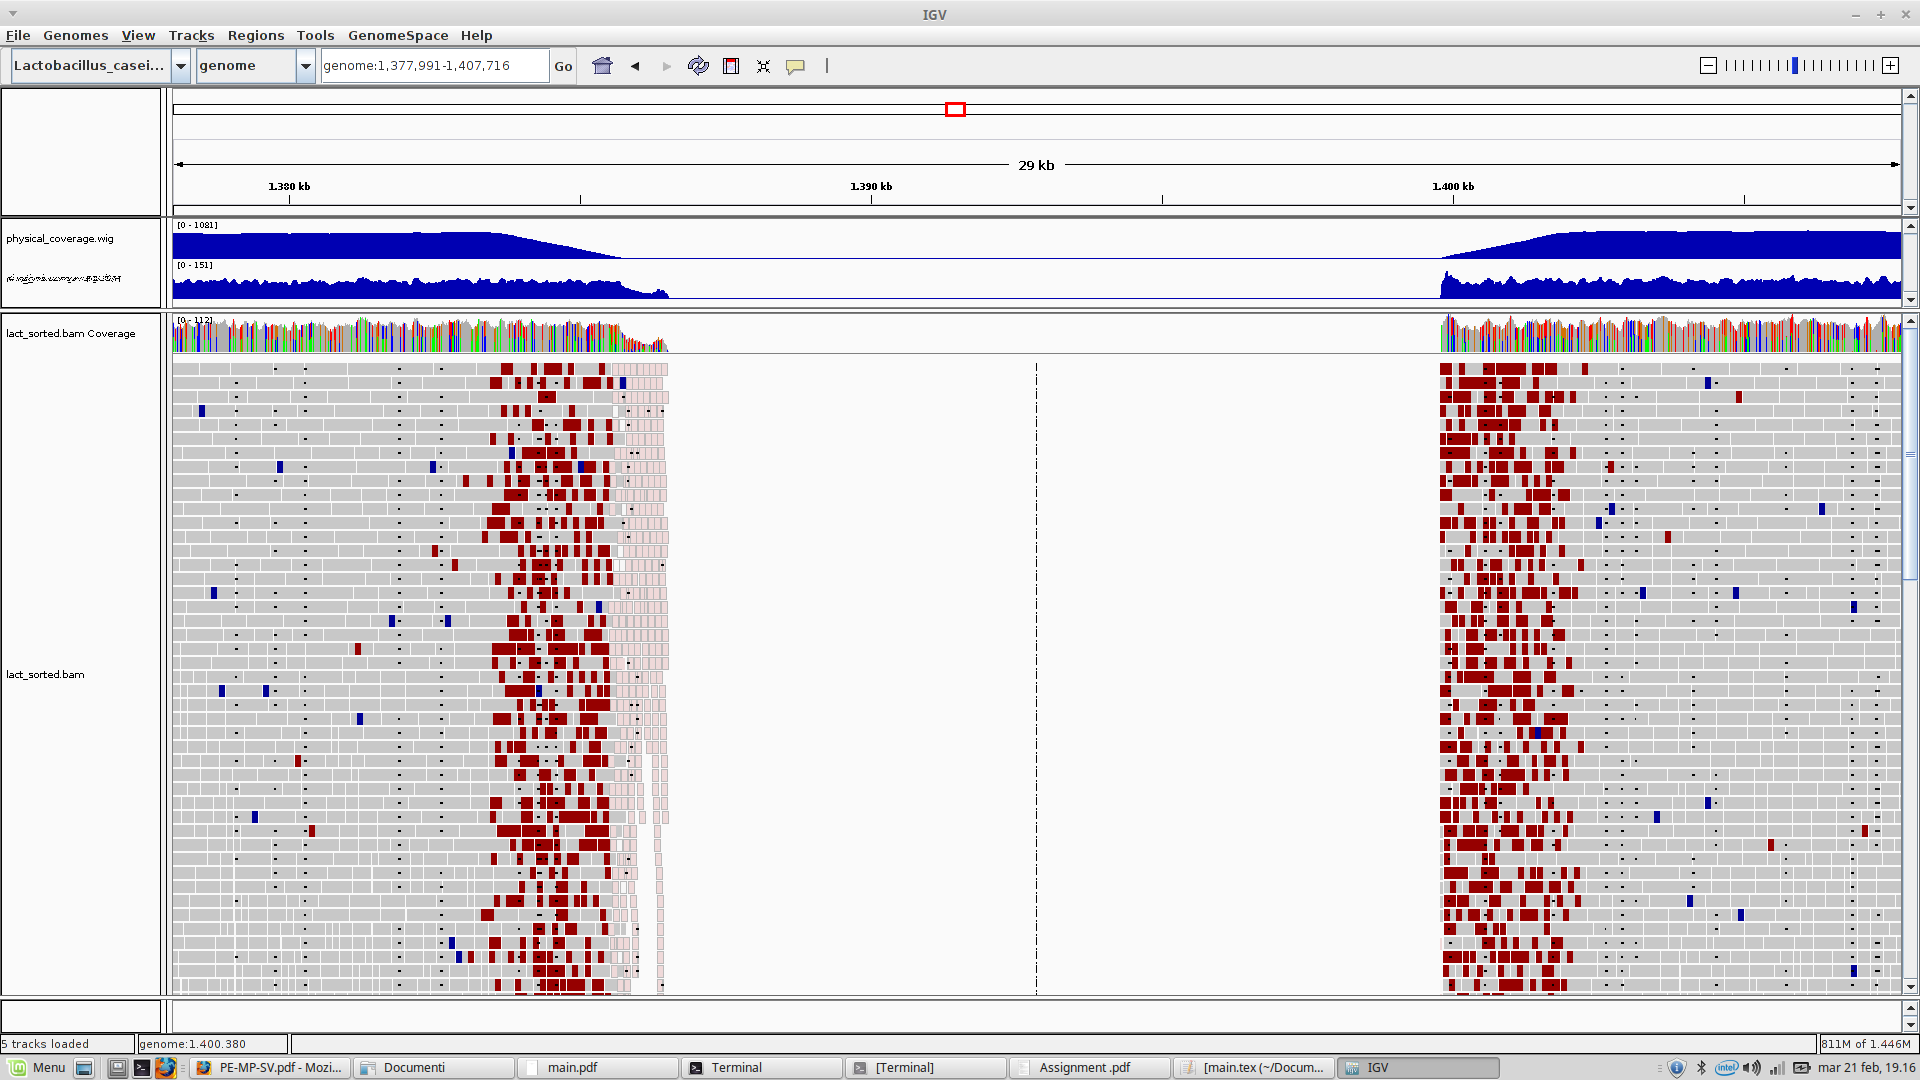
\includegraphics[scale=0.2]{img/pairs}
  \caption{Long deletion}
  \label{fig:pairs}
\end{figure}

In figure \ref{fig:small_del} there is a short deletion.

\begin{figure}[h]
  \centering
  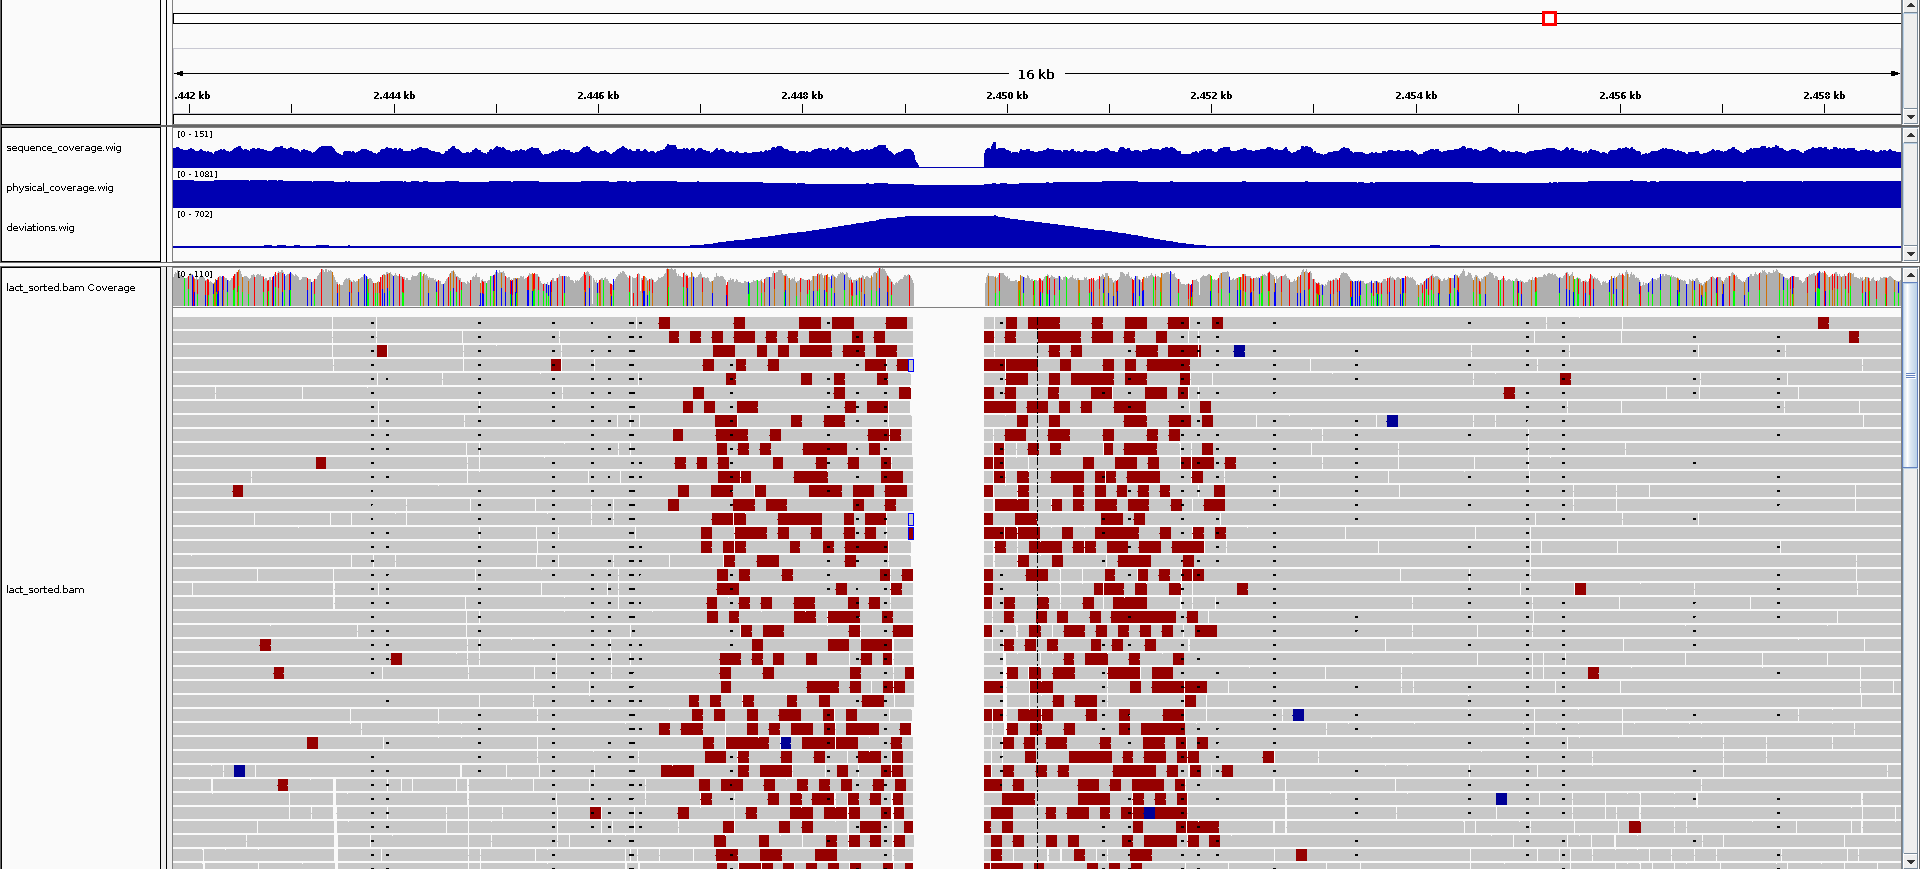
\includegraphics[scale=0.2]{img/small_del}
  \caption{Small deletion}
  \label{fig:small_del}
\end{figure}

In figure \ref{fig:long_insertion} there is a long insertion.

\begin{figure}[h]
  \centering
  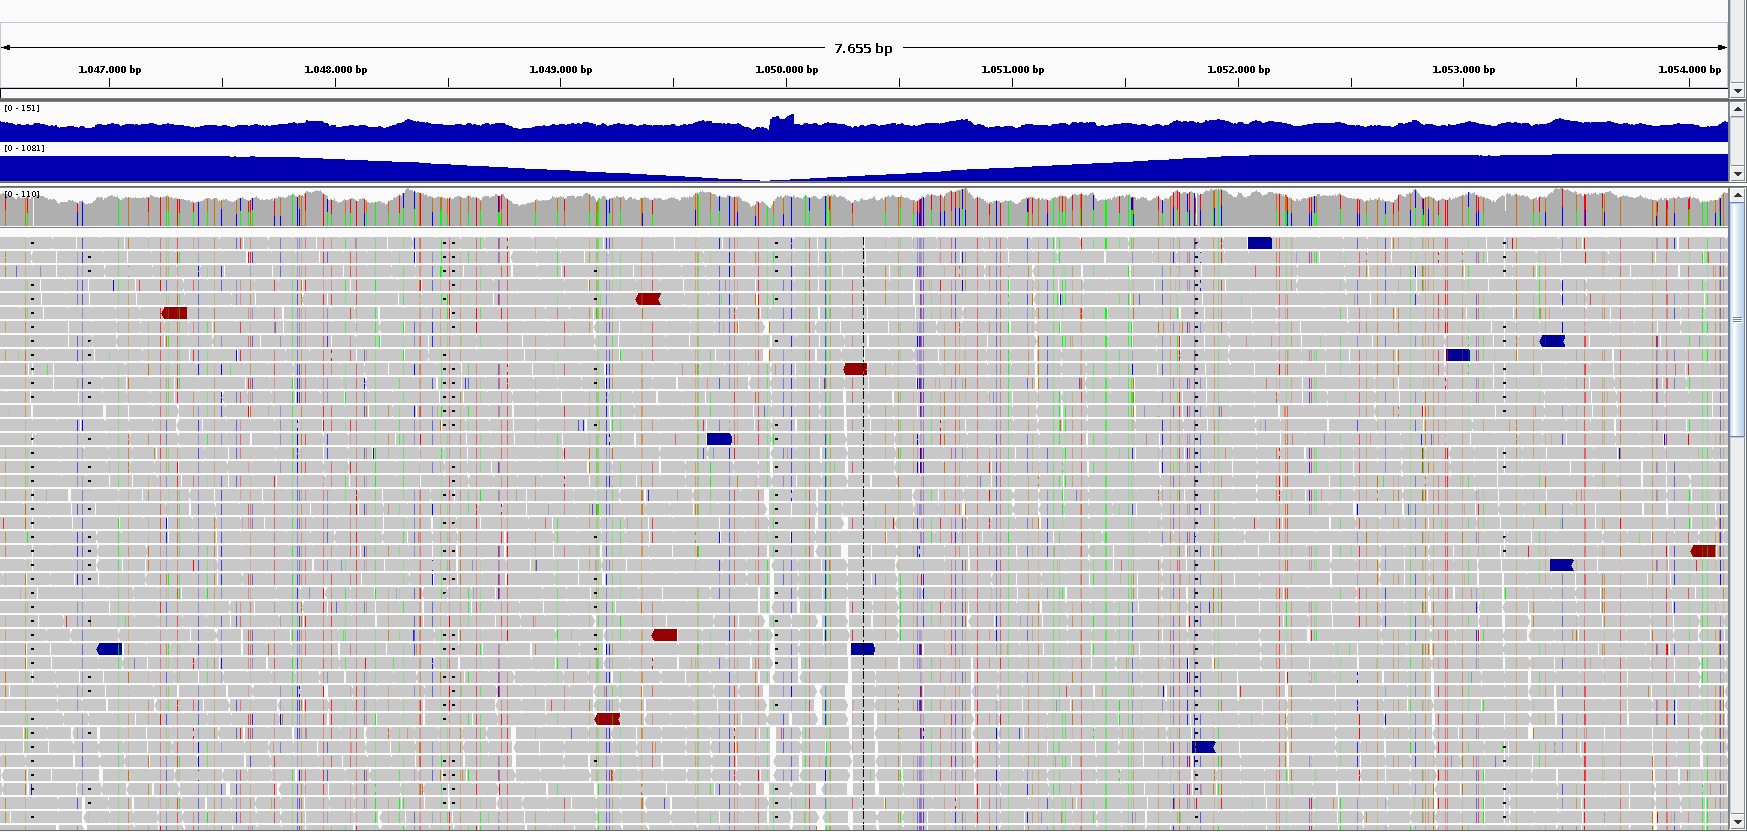
\includegraphics[scale=0.2]{img/long_insertion}
  \caption{Long insertion}
  \label{fig:long_insertion}
\end{figure}

\end{enumerate}

\newpage
\subsection{Part 2}

\begin{enumerate}
\setcounter{enumi}{8}
  \item Implement in the language of your choice a program to create a wig
file with physical covarage.
An example can be found in physical.pl, but it would be nice to implement
the suggestions described in physical\_coverage.pdf
  \item Create a wig track with sequence coverage and compare it with the
IGV track
  \item Read the sam file and for each mate pair calculate the length of the
genomic insert; then calculate the mean and standard deviation of the inserts,
possibly discarding those that are totally out of range
A plot of the length distribution may help to evaluate the sizes
  \item Create a track with the percentage of inserts with a length exceeding
n standard deviations (for instance n=2) above or below the mean
  \item Comment the results
\end{enumerate}

\subsection{Part 2 - Answers}

\begin{enumerate}
\setcounter{enumi}{8}
  \item Python script for physical coverage, given the sam file and
length of the reference genome:
\lstinputlisting[language=Python]{scripts/physical.py}
  \item Python script for sequence coverage, given the sam file and
length of the reference genome:
\lstinputlisting[language=Python]{scripts/sequence.py}
The wiggle file generates a track for sequence coverage and it is almost
similar to the IGV track.
So far the tracks created are the physical coverage and the genetic coverage:

\begin{figure}[h]
  \centering
  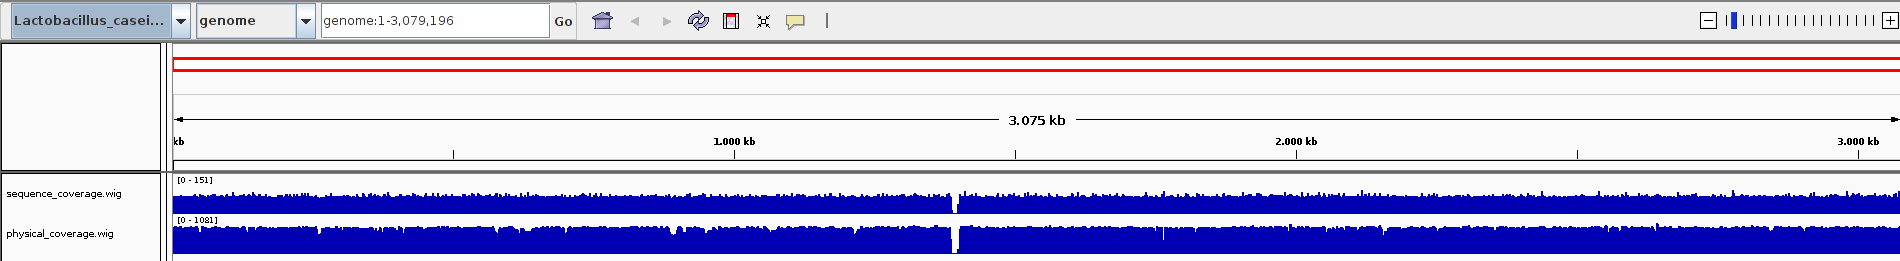
\includegraphics[scale=0.2]{img/ps_tracks}
  \caption{Physical and genetic coverage}
\end{figure}

  \item Python script to calculate the insert length, given the sam file and
length of the reference genome:
\lstinputlisting[language=Python]{scripts/insert.py}

In the previous calculation I assume that the two reads for a mate pair have
the same length.

So the length of the insert can be calculated by the following formula: \\

$matePos = Position\_of\_the\_mate$

$length = length\_of\_the\_aligned\_sequence$

$start = leftmost\_mapping\_position$ \\

$length\_of\_the\_insert = matePos + length - start$

\begin{figure}[h]
  \centering
  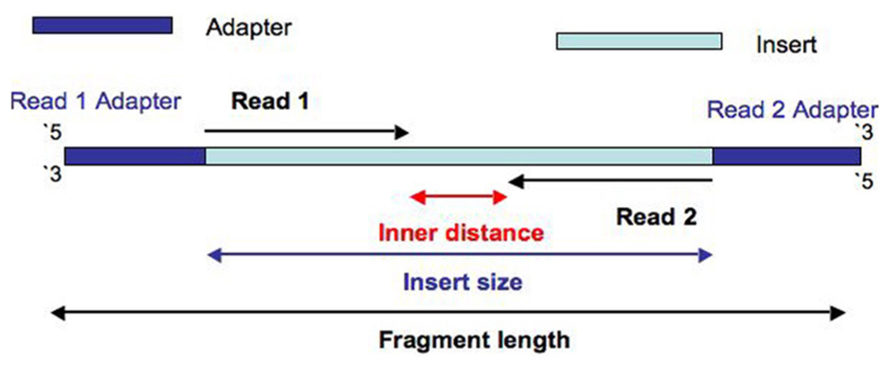
\includegraphics[scale=0.35]{img/insert_img}
  \caption{The length of the inserts has been calculated with this image as a reference}
\end{figure}

Python script to calculate the mean and the standard deviation, given the sam file,
length of the reference genome, the mean and the standard deviation.
\lstinputlisting[language=Python]{scripts/insert_mean_sd.py}

The mean is: \textbf{2220} \\

The standard deviation has been calculated by the formula: 

\begin{equation}
\sigma = \frac{1}{n}\sqrt{n*\sum_{i=1}^{n} x_i^2 - (\sum_{i=1}^{n} x_i)^2}
\end{equation}

and its value is: $\sigma = \textbf{203.495}$

  \item Python script to calculate the inserts above or below \textbf{(n = 2)} standard
deviation, given the wiggle file with the insert lengths:
\lstinputlisting[language=Python]{scripts/deviations.py}

In figure \ref{img:plot} are reported the length of the inserts (y axis) that are above/below
\textbf{n=3} standard deviation.
It can see that some insert are longer than 12000 bases.
The longest insert is 16281 bases long. \\

\begin{figure}[h]
  \centering
  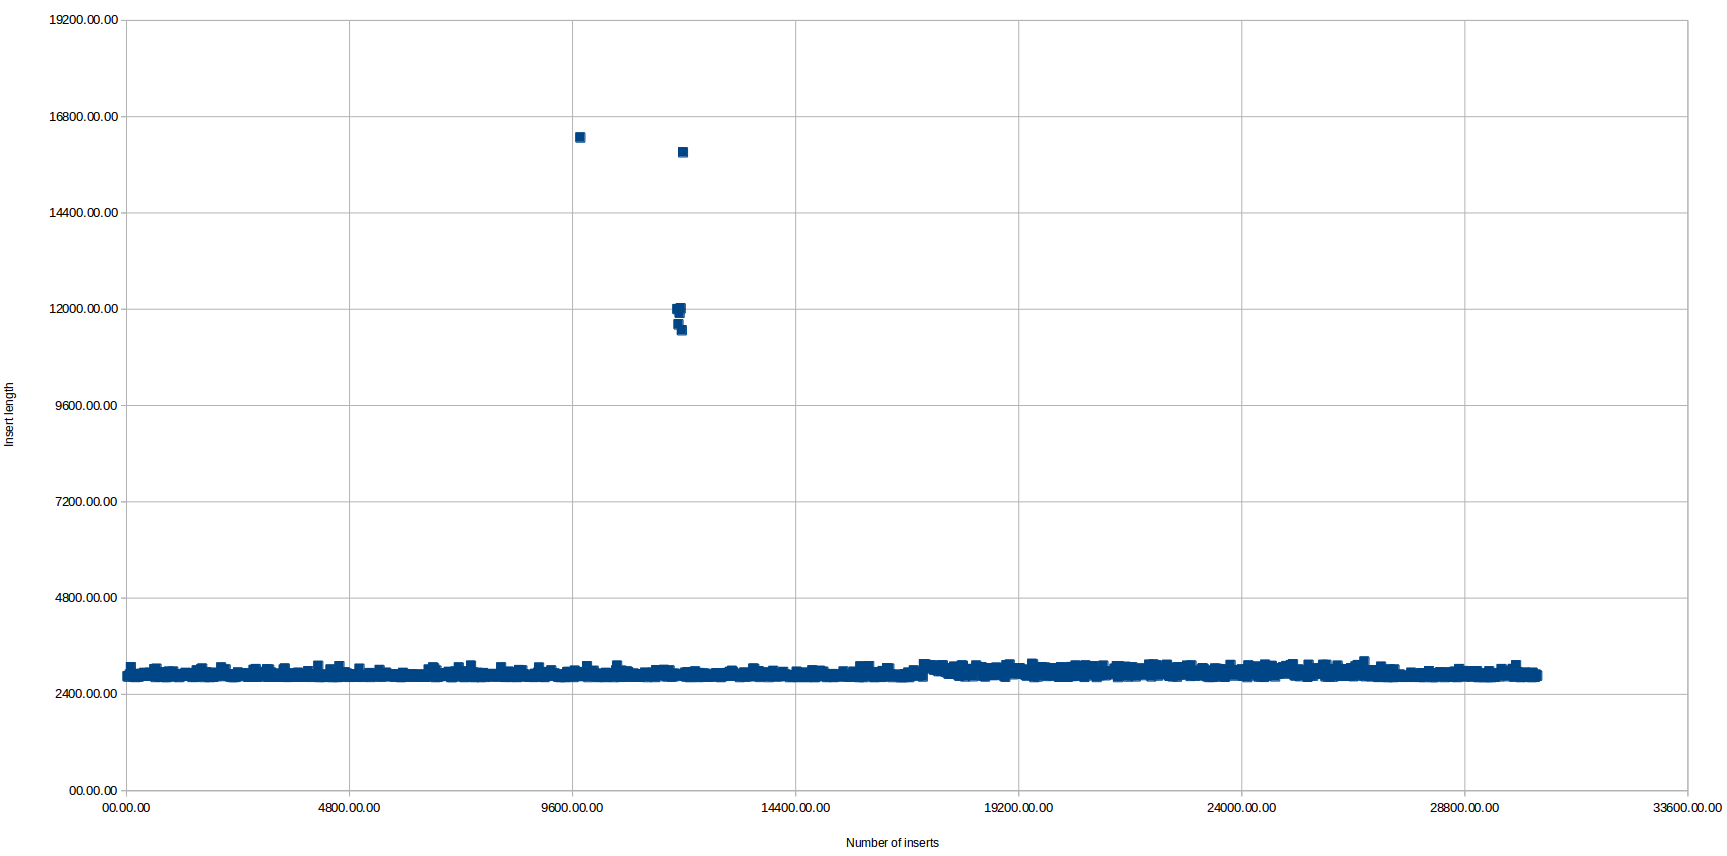
\includegraphics[scale=0.2]{img/plot}
  \caption{Plot for length of inserts}
  \label{img:plot}
\end{figure}

In figure \ref{img:all_tracks} all tracks from Part 2 of practicals can be seen. \\

\begin{figure}[h]
  \centering
  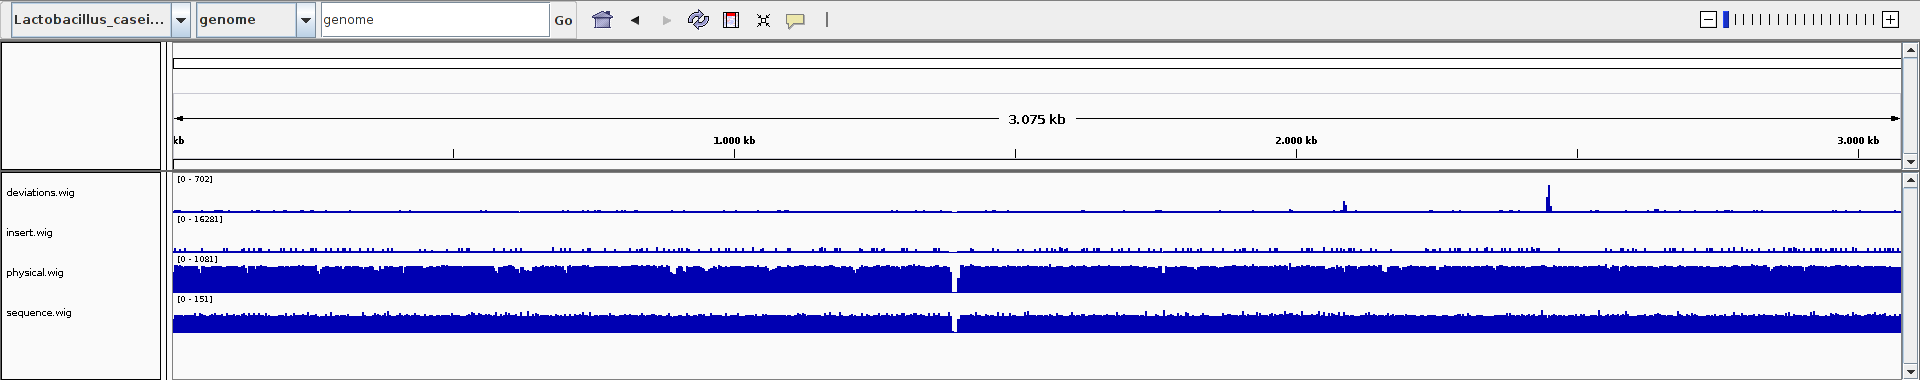
\includegraphics[scale=0.2]{img/all_tracks}
  \caption{All tracks required by Part 2 of practicals}
  \label{img:all_tracks}
\end{figure}

\newpage
\textbf{Observation on the scripts}: all the scripts are very short and simple
and they are thought to be used in the command line.
Almost every script uses an array that has the length of the reference genome.
This is very inefficient.

\newpage
\subsection{References}

In order to make Part 1 and Part 2 of practicals I used the following references:

\begin{itemize}
  \item \textbf{Mate-pairs and paired-ends} from the course slides
  \item \textbf{All the documents in the practicals directory} (unix.pdf, wig.pdf, physical.pdf)
  \item \textbf{IGV User Guide › Viewing Alignments › Interpreting Color by Insert Size}
\url{http://software.broadinstitute.org/software/igv/interpreting_insert_size}
  \item \textbf{Sequence Alignment/Map Format Specification} \url{http://samtools.github.io/hts-specs/SAMv1.pdf}
  \item \textbf{Decoding SAM flags} \url{https://broadinstitute.github.io/picard/explain-flags.html}
\end{itemize}

\end{enumerate}
